% Instrument control and HMI (formerly chapter9.tex)

% Chapter Template

%\section{Control Strategy} % Main chapter title

%\label{Chapter9} % For referencing this chapter elsewhere, use

%----------------------------------------------------------------------------------------
%\tSECTION 1
%----------------------------------------------------------------------------------------

\section{Control Strategy and Implementation}
\subsection{Modeling}

The project aims to implement a da Vinci–style surgical instrument claw effect using a compact 4-DoFs hardware architecture: a 3-DoFs manipulator arm plus a single gripper open/close degree of freedom. The system input is provided by the handle as three rotational joint angles and one gripper opening angle.

Since the manipulator itself has only three actual mechanical degrees of freedom, it cannot realize an arbitrary rotation axis in space. A specified direction in space requires three independent pose parameters, and a stable pose also consumes three degrees of freedom. This makes the system inherently over-constrained if arbitrary axis rotation is demanded. In contrast, the da Vinci system achieves effective 6-DOF stabilized control by using a larger arm to drive a smaller wristed arm in coordinated motion. Under the hardware constraints of this project, that six-degree-of-freedom stabilization strategy is not considered.

Instead, the control design adopts a decoupled attitude mapping. The coordinate system is defined using Euler angles to describe the desired end-effector orientation. The input attitude from the handle is mapped linearly to the output attitude of the manipulator, subject to the arm's three-degree-of-freedom limitations.


\subsection{Denavit–Hartenberg Coordinate Frames}
The coordinate frames are established using standard Denavit–Hartenberg conventions, as shown in Figures~\ref{fig:dhcord} and~\ref{fig:dhcord1}. The manipulator consists of three rotary joints, with the following D-H parameters:

\begin{table}[htbp]
    \centering
    \caption{Denavit–Hartenberg parameters for the 3-DoF manipulator}
    \label{tab:dhparams}
    \begin{tabular}{c c c c c l}
        \toprule
        Link & $\theta_i$ & $d_i$ & $a_i$ & $\alpha_i$ & Remarks \\
        \midrule
        1 & \(\theta_1\) & 0 & 0 & \(-90^\circ\) & Base rotation \\
        2 & \(90^\circ - \theta_2\) & 0 & \(-a_2\) & \(90^\circ\) & Upper arm rotation \\
        3 & \(\theta_3 - 180^\circ\) & 0 & \(a_3\) & 0 &  \\
        \bottomrule
    \end{tabular}
\end{table}

And the following Rotation Matrix for the end-effector orientation:
\[
A_1 =
\begin{bmatrix}
c_1 & 0 & -s_1 & 0 \\
s_1 & 0 & c_1 & 0 \\
0 & -1 & 0 & 0 \\
0 & 0 & 0 & 1
\end{bmatrix},
\qquad
A_2 =
\begin{bmatrix}
s_2 & 0 & c_2 & -a_2 s_2 \\
c_2 & 0 & -s_2 & -a_2 c_2 \\
0 & 1 & 0 & 0 \\
0 & 0 & 0 & 1
\end{bmatrix},
\qquad
A_3 =
\begin{bmatrix}
-c_3 & -s_3 & 0 & -a_3 c_3 \\
s_3 & -c_3 & 0 & a_3 s_3 \\ 
0 & 0 & 1 & 0 \\
0 & 0 & 0 & 1
\end{bmatrix}
\]
The end-effector pose is governed by the following equations:
\begin{align*}
P_x &= c_1 s_2(-a_3 c_3) + (-s_1)(a_3 s_3) + c_1 c_2(0) + (-a_2 c_1 s_2) \\
& \rightarrow P_x= -a_3 c_1 s_2 c_3 - a_3 s_1 s_3 - a_2 c_1 s_2 \\
P_y &= s_1 s_2(-a_3 c_3) + c_1(a_3 s_3) + s_1 c_2(0) + (-a_2 s_1 s_2) \\
& \rightarrow P_y= -a_3 s_1 s_2 c_3 + a_3 c_1 s_3 - a_2 s_1 s_2 \\
P_z &= -c_2(-a_3 c_3) + 0(a_3 s_3) + s_2(0) + a_2 c_2 \\
& \rightarrow P_z= a_3 c_2 c_3 + a_2 c_2
\end{align*}
The orientation of the end effector can also be expressed through the base axis direction vectors shown in Table~\ref{tab:axisdir}.

\begin{table}[htbp]
\centering
\caption{End-effector base-axis direction vectors}
\label{tab:axisdir}
\begin{tabular}{|l|l|l|l|}
\hline
\textbf{Direction} & \textbf{X-axis  ($n$)} & \textbf{Y-axis  ($o$)} & \textbf{Z-axis  ($a$)} \\
\hline
Base X-axis & $-c_1 s_2 c_3 - s_1 s_3$ & $-c_1 s_2 s_3 + s_1 c_3$ & $c_1 c_2$ \\
\hline
Base Y-axis & $-s_1 s_2 c_3 + c_1 s_3$ & $-s_1 s_2 s_3 - c_1 c_3$ & $s_1 c_2$ \\
\hline
Base Z-axis & $c_2 c_3$ & $c_2 s_3$ & $s_2$ \\
\hline
\end{tabular}
\end{table}

\begin{figure}[htbp]
    \centering
    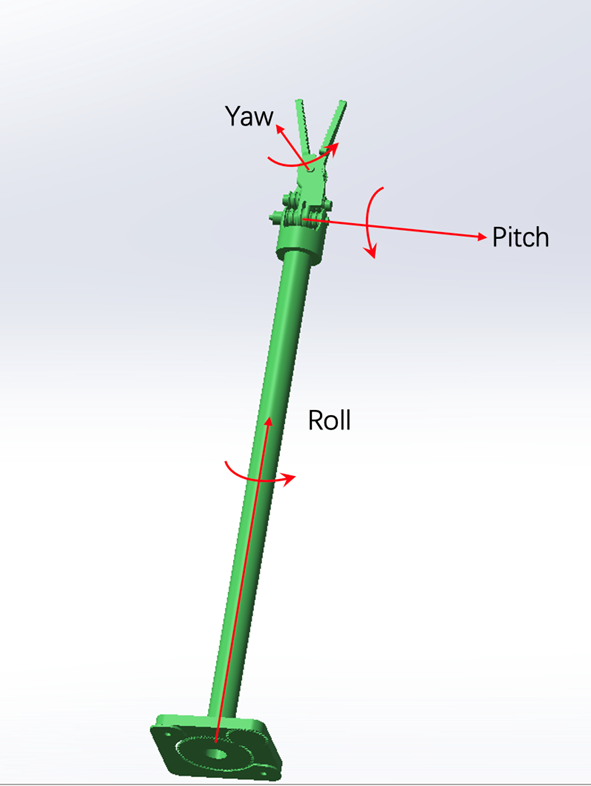
\includegraphics[width=0.8\linewidth]{Figures/DH cord1.png}
    \caption{Denavit–Hartenberg coordinate frame definition for the manipulator}
    \label{fig:dhcord}
\end{figure}

\begin{figure}[htbp]
    \centering
    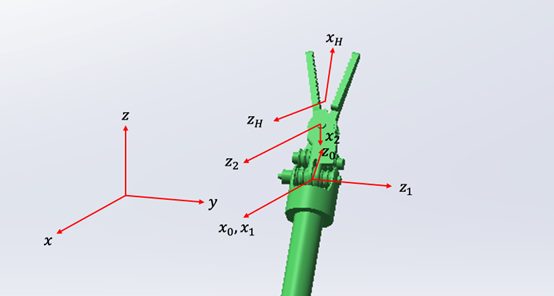
\includegraphics[width=0.8\linewidth]{Figures/DH cord.png}
    \caption{Alternative view of the D-H coordinate frames and joint axes}
    \label{fig:dhcord1}
\end{figure}

\subsection{System Architecture and Data Flow}
The control system is implemented on an ESP32 microcontroller running FreeRTOS, enabling real-time processing of sensor inputs and actuator commands. The architecture follows a cyclic loop structure, as illustrated in the firmware code, where sensor feedback is continuously acquired, processed, and translated into motor commands.

At the core of the system is a feedback loop that reads position, speed, load, voltage, temperature, and current from eight Feetech STS-series servos via UART communication. This multi-modal feedback provides the foundation for state estimation and control. The input module captures user intent through four degrees of freedom: wrist yaw, pitch, roll, and gripper opening/closing, using AS5600 magnetic encoders and STS3009 servos for precise motion detection.

\subsection{Intent Estimation and Command Mapping}
User inputs are mapped from encoder readings to angular commands. The firmware calculates roll, pitch, yaw, and gripper commands by scaling encoder positions relative to a midpoint. For instance, $roll_cmd$ is derived from the difference between encoder p8 and the midpoint, scaled to degrees. These commands are then transformed into servo-specific inputs, accounting for mechanical ratios and phase offsets to ensure coordinated motion.

The transformation incorporates kinematic considerations, such as the differential yaw control for the gripper jaws, where $s3\_yaw\_right$ and $s4\_yaw\_left$ are adjusted based on $yaw\_in$ and $gripper\_cmd$ to achieve symmetric or asymmetric grasping.

To robustly infer operator intent in the presence of noise and delay, an Extended Kalman Filter (EKF) can be integrated as a future enhancement. The EKF would fuse sensor inputs from AS5600 encoders, motor encoders, and optional inertial measurements from an IMU module. It maintains estimates of finger poses, wrist orientation, and cable tensions, enabling predictive control and improved stability during rapid transitions. This probabilistic approach handles uncertainties in sensor readings, providing smoother and more reliable command generation compared to the current direct mapping.

\subsection{Low-Level Actuation and Tension Management}
Actuation is handled through direct position control of the STS3032 servos for the output stage and STS3009 for input stabilization. The code implements a locking mechanism for the gripper motors: when the gripper is open beyond a threshold $(gripper_open = 5.0 degrees)$, the motors are unloaded to reduce power consumption and allow free motion; otherwise, they are locked to maintain tension.

This tension management is critical for cable-driven systems, preventing slack while enabling compliant interaction. The firmware uses the servo's built-in position mode with zero speed and acceleration for precise control, ensuring smooth transitions without oscillations.

\subsection{System Implementation and Details}
Safety is ensured through conditional motor unloading and error management. When feedback faults occur—such as communication dropouts—the system illuminates an error LED and stops execution. At startup, a homing routine moves the servos to their neutral positions, enabling the encoders to establish reference baselines.

While running, the lock/release mechanism functions as a safety measure: it relieves cable tension whenever the gripper is open, preventing unintended forces on tissue.

Visual and diagnostic feedback is delivered through a WS2812 LED strip and serial output. Error conditions activate red LEDs, whereas normal operation leaves the indicators off. Both USB and Bluetooth connectivity support data logging, facilitating offline analysis of control performance and user interactions.

The firmware communicates with servos via HardwareSerial at 500k baud and uses standard Serial for debugging. Motor commands are assembled using a custom protocol that includes unload/enable directives. The main loop executes roughly every 3 ms, striking a balance between system responsiveness and computational overhead.

This implementation embodies a practical tendon-driven control framework, translating high-level intentions into low-level actuation while emphasizing safety and usability within a compact, real-time system.
